\documentclass[12pt]{article}
\usepackage[a4paper,margin=1in]{geometry}
\usepackage{enumitem}
\usepackage{graphicx}
\usepackage{hyperref}
\usepackage{longtable}
\usepackage{float}

\title{Lab Assignment 3}
\author{Deepak Sarun Yuvachandran}
\date{November 17th 2024}


\begin{document}

\maketitle


\section*{Task 1: Set Up the Dev Environment}

\subsection*{(1) Screenshots of Your App}

\textbf{App running in emulator:}
\begin{center}
    
\includegraphics[width=0.5\textwidth, height=16cm]{images/emulator.png.jpg} 
\end{center}

\textbf{App running in physical device:}
\begin{center}
    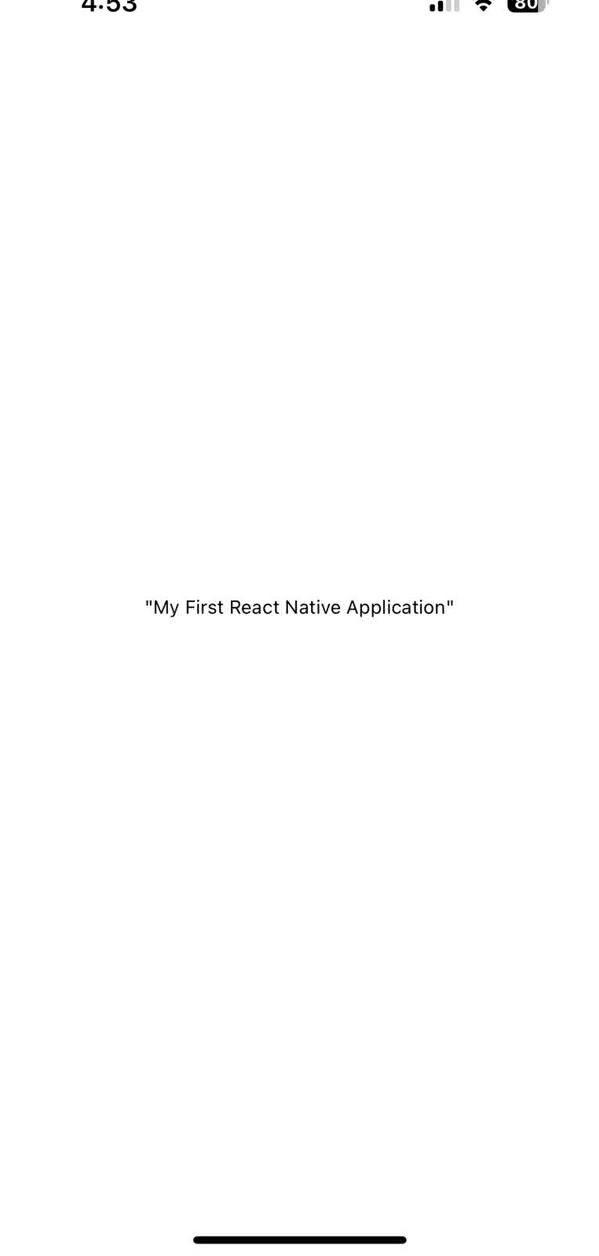
\includegraphics[width=0.5\textwidth, height=16cm]{images/physicaldevice.png} 
\end{center}

\subsection*{Differences Observed}
\begin{itemize}
    \item \textbf{Performance:} Apps on the emulator may experience lag, especially with animations or intensive operations, while physical devices typically run smoother.
    \item \textbf{Hardware-Specific Features:} Testing GPS, camera, or accelerometer functionality is more reliable on a physical device. Emulators may simulate these but lack accuracy.
    \item \textbf{Screen Resolution:} Physical devices give a true representation of the display, whereas emulator scaling might vary.
    \item \textbf{Input Mechanism:} On emulators, interactions are simulated via a mouse or keyboard, whereas physical devices rely on real touch gestures.
\end{itemize}

\subsection*{(2) Setting Up an Emulator}

\paragraph{Detailed Steps to Set Up an Emulator in Android Studio:}
\begin{enumerate}
    \item \textbf{Install Required Tools:} Download and install Android Studio from \url{https://developer.android.com/studio}. Ensure you install the Android SDK during the initial setup.
    \item \textbf{Open the Device Manager:} Navigate to \texttt{Tools > Device Manager} in Android Studio. Alternatively, use the shortcut from the toolbar.
    \item \textbf{Create a New Virtual Device:}
    \begin{enumerate}[label*=\arabic*.]
        \item Click ``Create Device''.
        \item Select the desired hardware profile.
        \item Review specifications such as screen size, resolution, and RAM.
    \end{enumerate}
    \item \textbf{Select a System Image:} Choose the target API level (API 35 for Android 15). Download the system image if not already available.
    \item \textbf{Configure Emulator Settings:} Adjust options such as startup orientation, RAM allocation, and virtual SD card size. Enable or disable camera and microphone simulation.
    \item \textbf{Launch the Emulator:} Start the emulator by clicking the play button in the Device Manager.
\end{enumerate}

\subsection*{Tips for Emulator Optimization}
\begin{itemize}
    \item Use Quick Boot for faster subsequent launches.
    \item Enable GPU Acceleration: Go to \texttt{Preferences > Emulator} and enable hardware-accelerated graphics.
    \item Increase RAM Allocation for faster app load times.
\end{itemize}

\subsection*{Challenges and How to Overcome Them}
\begin{itemize}
    \item \textbf{Emulator Freezes or Crashes:}
    \begin{itemize}
        \item Check virtualization (Intel VT-x/AMD-V) is enabled in BIOS.
        \item Update GPU drivers for compatibility.
    \end{itemize}
    \item \textbf{HAXM Installation Error:} Install HAXM manually from the Android Studio SDK Manager. For Windows users, enable Hyper-V in \texttt{ Control Panel > Programs > Turn Windows Features On/Off}.
    \item \textbf{Slow Startup:} Reduce emulator resolution to a lower DPI.
\end{itemize}

\subsection*{(3) Running the App on a Physical Device Using Expo}

\paragraph{Detailed Steps to Connect a Physical Device:}
\begin{enumerate}
    \item Install Node.js and ensure it is the latest LTS version.
    \item Install Expo CLI: \texttt{npm install -g expo-cli}
    \item Initialize Your React Native Project:
    \begin{verbatim}
expo init my-app
cd my-app
    \end{verbatim}
    \item Run the Expo Development Server:
    \begin{verbatim}
expo start
    \end{verbatim}
    \item Download the Expo Go app and scan the QR code displayed in the terminal.
\end{enumerate}

\subsection*{Troubleshooting Steps for Physical Device Setup}
\begin{itemize}
    \item \textbf{App Fails to Load:}
    \begin{itemize}
        \item Run \texttt{expo doctor} for diagnosing dependency issues.
        \item Ensure the physical device and development machine are on the same Wi-Fi network.
    \end{itemize}
    \item \textbf{Network Problems:} Switch to LAN or USB debugging using the Expo development tools.
    \item \textbf{Cache Problems:} Clear Metro bundler cache:
    \begin{verbatim}
expo start --clear
    \end{verbatim}
    \item Use the Expo app to test push notifications, media, and performance.
\end{itemize}

\subsection*{(4) Comparison of Emulator vs. Physical Device}

\begin{table}[H]  % Use table with [H] to keep the table in place
\centering
\renewcommand{\arraystretch}{1} % Adjust row height
\setlength{\tabcolsep}{10pt} % Adjust column spacing
\begin{tabular}{|p{4cm}|p{5cm}|p{5cm}|}
\hline
\textbf{Criteria} & \textbf{Emulator} & \textbf{Physical Device} \\ \hline
Setup Requirements & 
Requires Android Studio or Xcode installation and configuration. & 
Requires enabling developer mode, USB debugging (Android), or provisioning profiles (iOS). \\ \hline
Performance & 
May lag, especially on low-spec machines. & 
Generally smoother and closer to real-world performance. \\ \hline
Device Diversity & 
Can simulate multiple devices, screen sizes, and OS versions easily. & 
Limited to devices you physically own. \\ \hline
Realism & 
Simulated gestures and hardware interactions (e.g., GPS, camera). & 
Real touch responsiveness and accurate hardware testing. \\ \hline
Debugging Tools & 
Preloaded debugging tools (e.g., layout inspector, memory profiler). & 
Limited debugging; requires external tools (e.g., React Native Debugger). \\ \hline
Resource Usage & 
High CPU and RAM usage; requires virtualization enabled on the host machine. & 
Minimal resource impact on the development machine. \\ \hline
Hardware-Specific Testing & 
Limited; simulated hardware behavior may not match real devices. & 
Accurate testing of hardware features like accelerometer, camera, and sensors. \\ \hline
Ease of Use & 
Easy to test across various configurations without owning multiple devices. & 
Requires manual switching between physical devices. \\ \hline
Network Testing & 
Simulates various network conditions but may not replicate real-world usage. & 
Real-world network conditions provide accurate behavior testing. \\ \hline
Cost & 
Free; no need to buy devices. & 
Requires investment in physical devices. \\ \hline
Battery Testing & 
Allows simulation of different battery states (low, charging, etc.). & 
Real battery performance testing under actual usage conditions. \\ \hline
User Experience Testing & 
Limited; lacks actual user interaction feedback. & 
Real-world testing with accurate feedback on gestures and navigation. \\ \hline
Best Use Cases & 
Initial testing, layout debugging, layout and screen sizes. & 
Final testing, performance evaluation, and accurate testing. \\ \hline
\end{tabular}
\caption{Comparison of Emulator vs. Physical Device}
\label{tab:comparison}
\end{table}

\subsection*{(5) Troubleshooting a Common Error}
\paragraph{Error:} ``Unable to resolve module .''

\paragraph{Cause:} Missing package, improper linking, or compatibility issues.

\paragraph{Steps to Resolve:}
\begin{itemize}
    \item Check if the module is installed:
    \begin{verbatim}
npm list module-name
    \end{verbatim}
    \item If not, install it:
    \begin{verbatim}
npm install module-name
    \end{verbatim}
    \item Clear cache and rebuild the project:
    \begin{verbatim}
npm start --reset-cache
    \end{verbatim}
    \item Verify compatibility of React Native version with the module.
\end{itemize}

\section*{Task 2: Building a Simple To-Do List App}

\subsection*{(a) Mark Tasks as Complete}

\paragraph{Toggle Function for Marking Tasks as Completed:}
The \texttt{toggleTaskCompletion} function is responsible for toggling the \texttt{completed} status of tasks. When a user clicks the "Complete" button, it toggles the task's completion state.
\begin{center}
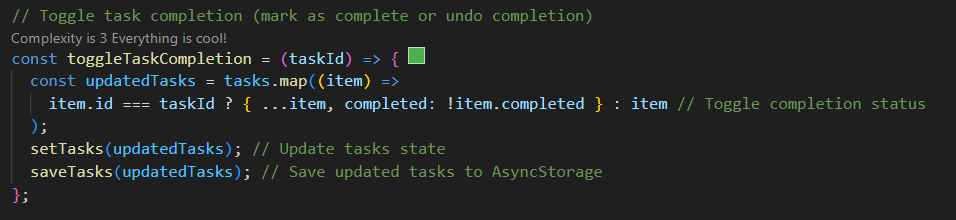
\includegraphics[width=1\textwidth]{images/completedtoggle.png} 
\end{center}
\paragraph{Styling Completed Tasks Differently:}
When a task is marked as completed:
\begin{itemize}
    \item The text gets a strikethrough.
    \item The color changes to gray using conditional styling.
\end{itemize}
\begin{center}
    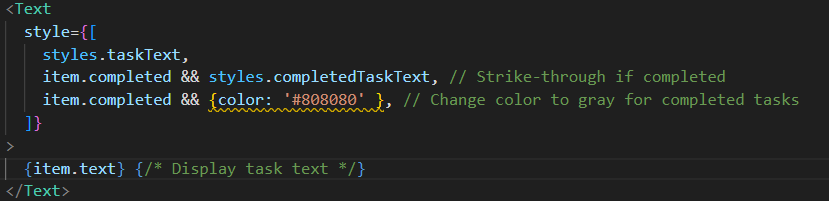
\includegraphics[width=1\textwidth, height=5cm]{images/stylecompletedtask.png} 
\end{center}

\paragraph{Explanation:}
The \texttt{completed} property in each task object is toggled between \texttt{true} and \texttt{false}. This change is reflected in the state by using the \texttt{setTasks} function, which updates the tasks array. The \texttt{saveTasks} function ensures the updated list is saved to \texttt{AsyncStorage}, so the completion status persists across app restarts.

\textbf{Example of a completed task:}
\begin{itemize}
    \item \texttt{food} is marked as a completed task.
\end{itemize}

\textbf{Screenshot of Marking Tasks as Complete:}
\begin{center}
    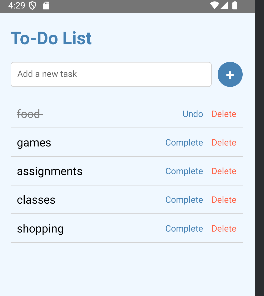
\includegraphics[width=0.5\textwidth, height=12cm]{images/completedtask3.png} 
\end{center}

\subsection*{(b) Persist Data Using AsyncStorage}

\paragraph{Implementing Data Persistence:}
\texttt{AsyncStorage} is used to persist the tasks so that they remain saved even after the app is closed and reopened.

\paragraph{Functions:}
\begin{itemize}
    \item \texttt{loadTasks}: Retrieves the tasks from \texttt{AsyncStorage}.
    \item \texttt{saveTasks}: Stores the tasks in \texttt{AsyncStorage}.
\end{itemize}

\paragraph{Explanation:}
When the app is launched, the tasks are loaded from \texttt{AsyncStorage} by calling \texttt{loadTasks} inside the \texttt{useEffect} hook. This ensures the task list is available on startup. When a task is added, deleted, or edited, the updated task list is saved back to \texttt{AsyncStorage} using \texttt{saveTasks}.

\textbf{Screenshot of Data Persistence:}
\begin{center}
    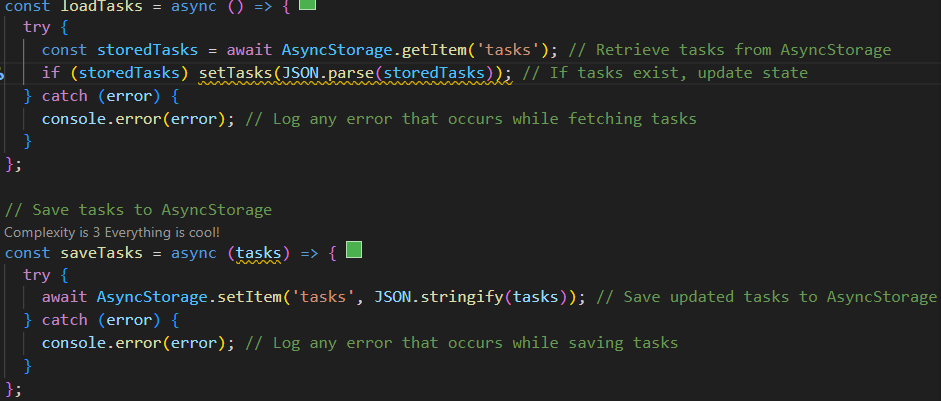
\includegraphics[width=0.9\textwidth, height=6cm]{images/async.png} 
\end{center}

\subsection*{(c) Edit Tasks}

\paragraph{Allow Users to Tap on a Task to Edit:}
The \texttt{openEditModal} function opens a modal with the current task's content when a user taps on a task. The input field in the modal is pre-filled with the task's text, allowing the user to edit it.
\begin{center}
    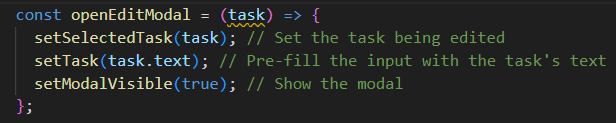
\includegraphics[width=\textwidth, height=3cm]{images/edittask1.png} 
\end{center}
\paragraph{Update Function to Modify Task in the State:}
When the user saves the edited task, the \texttt{editTask} function updates the task in the \texttt{tasks} state array and saves it to \texttt{AsyncStorage}.
\begin{center}
    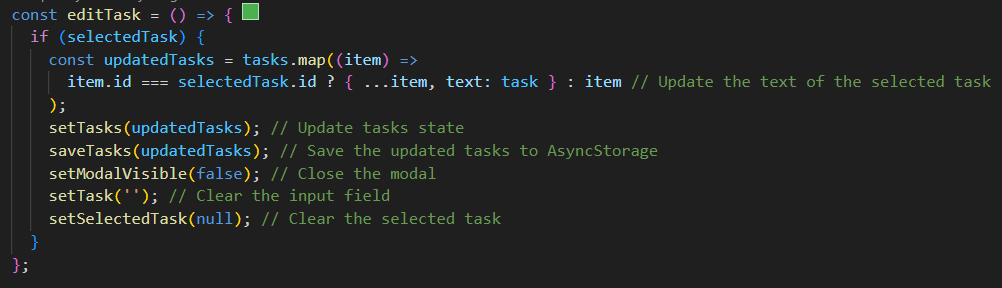
\includegraphics[width=\textwidth, height=6cm]{images/edittask2.png} 
\end{center}

\paragraph{Explanation:}
The state is updated by mapping through the \texttt{tasks} array and modifying the text of the selected task. This ensures the task is updated in the state, and the new list is saved in \texttt{AsyncStorage} for persistence.

\textbf{Screenshot of Editing Tasks:}
\begin{center}
    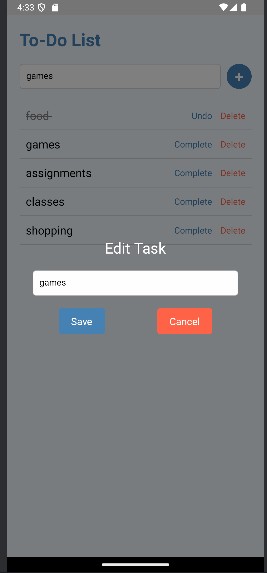
\includegraphics[width=0.6\textwidth, height=15cm]{images/edittask3.png} 
\end{center}

\subsection*{(d) Add Animations}

\paragraph{Using the Animated API:}
The \texttt{Animated} API is used to add an animation effect when a task is added to the list. This animation enlarges the "Add" button briefly to provide feedback when a task is added.

\begin{verbatim}
const spider = new Animated.Value(0); // Create animation value
\end{verbatim}
\begin{center}
    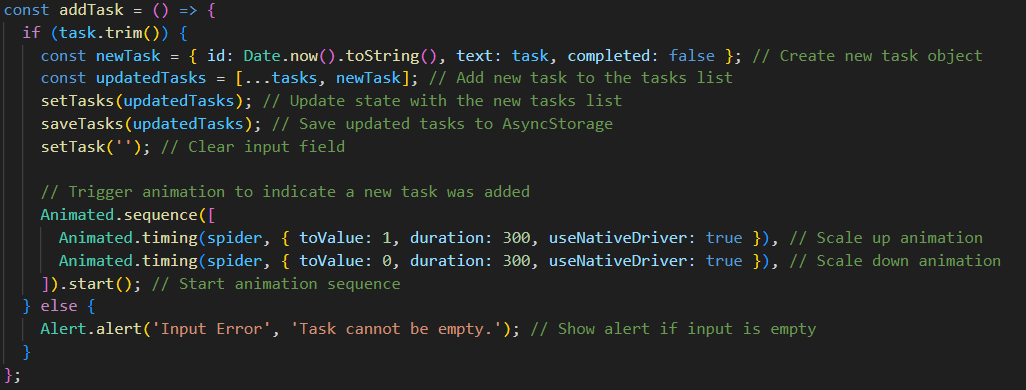
\includegraphics[width=\textwidth, height=6cm]{images/animation1.png} 
\end{center}

\paragraph{Animation Style:}
The animated style for the "Add" button is applied through \texttt{Animated.Text} and uses the \texttt{scale} transform to provide a visual feedback when a task is added.
\begin{center}
    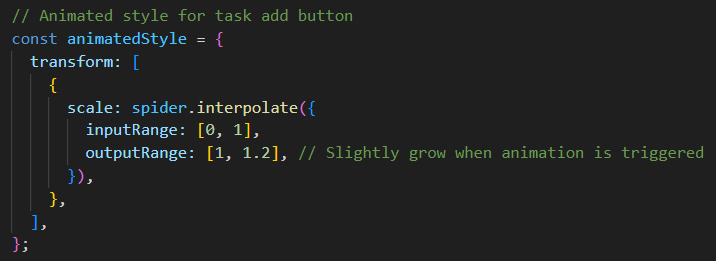
\includegraphics[width=\textwidth, height=8cm]{images/animated2.png} 
\end{center}
\paragraph{Explanation:}
The animation is triggered when a new task is added. It scales the "Add" button up briefly (to 1.2 times its size) and then shrinks it back to its original size. This gives users feedback that their action has been registered. The \texttt{Animated.Value} is used to control the animation’s state, and \texttt{Animated.timing} is used to change the value over time.

\textbf{Screenshot of Animation Effect:}
\begin{center}
    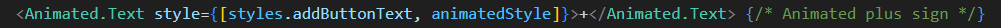
\includegraphics[width=1\textwidth, height=0.6cm]{images/animated3.png} 
\end{center}

\begin{center}
    \section*{ \href{https://github.com/DeeapakSarun/ToDoApp.git}{GitHub Project Link}}
\end{center}

\end{document}